\documentclass[journal=jpccck,manuscript=article]{achemso}

\usepackage{hyperref}

\usepackage{siunitx}
\DeclareSIUnit\rydberg{Ry}
\usepackage{tikz}
\usepackage{paralist}
\usepackage[version=4]{mhchem}
\usepackage{booktabs}
\usepackage{rotating}
\usepackage{chngcntr}


\author{Pierre Beaujean}
\affiliation[Unamur]
{University of Namur, Theoretical Chemistry Lab, Unit of Theoretical and Structural Physical Chemistry, Namur Institute of Structured Matter, rue de Bruxelles, 61, B-5000 Namur (Belgium)}


\author{Benoît Champagne}
\affiliation[Unamur]
{University of Namur, Theoretical Chemistry Lab, Unit of Theoretical and Structural Physical Chemistry, Namur Institute of Structured Matter, rue de Bruxelles, 61, B-5000 Namur (Belgium)}
\email{benoit.champagne@unamur.be}

\title{Prediction of XPS binding energies for molecules grafted on calcium surfaces\\Supporting information}

\def\dbe{\ensuremath{\Delta\text{BE}}}



\renewcommand{\thetable}{S\arabic{table}}
\renewcommand{\thefigure}{S\arabic{figure}}

\begin{document}
	\maketitle

\begin{figure}[!h]
	\centering
	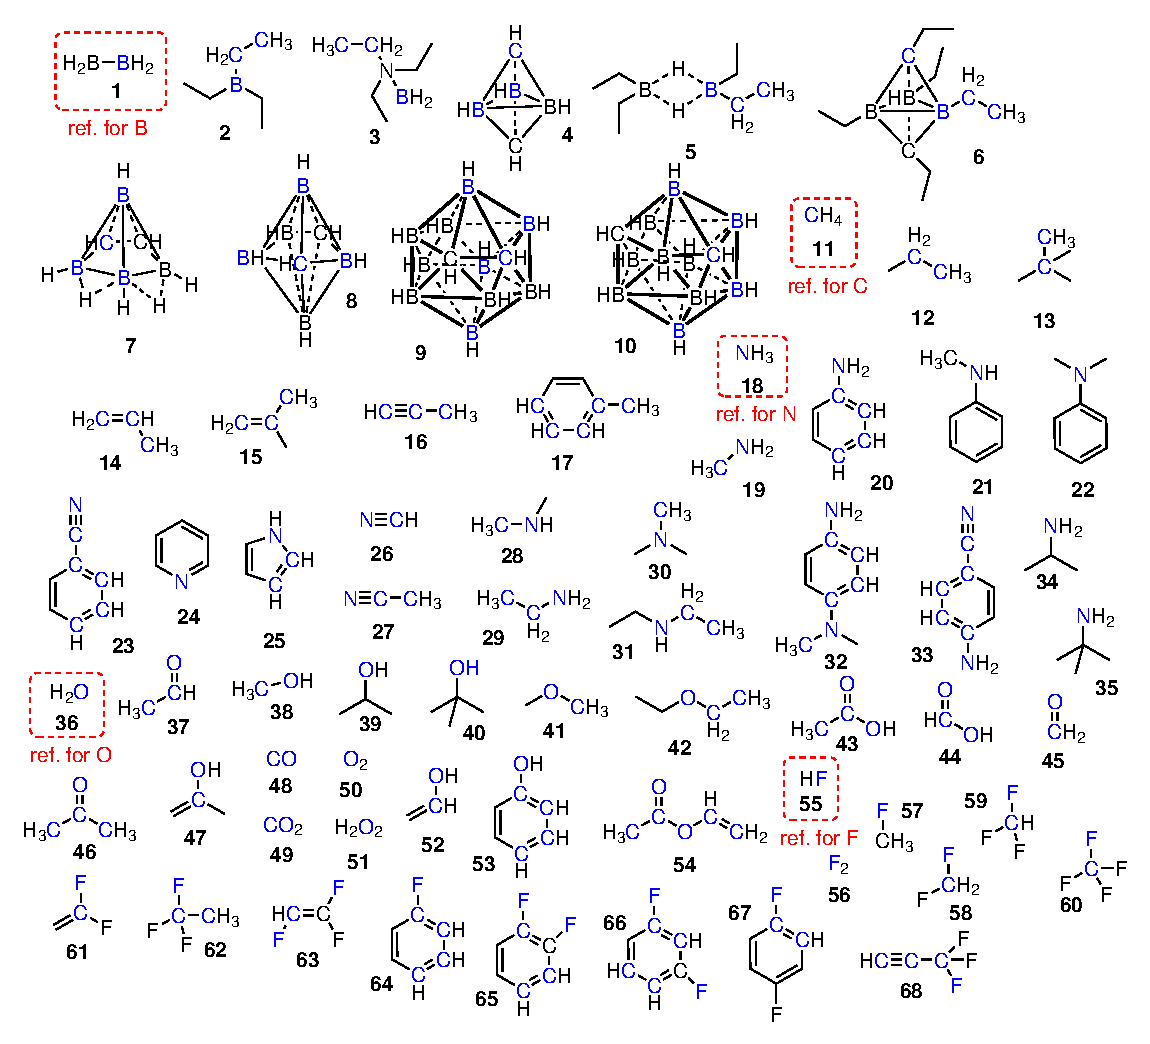
\includegraphics[width=\linewidth]{FigureS1}
	\caption{Molecules for the benchmark , from Ref.~\citenum{pueyobellafontPredictingCoreLevel2017}. The atoms for which experimental BE are provided are highlighted in blue.  The reference compounds used for each atom are highlighted in red.}
	\label{fig:core185}
\end{figure}


\begin{figure}[!h]
	\includegraphics[width=\linewidth]{FigureS2}
	\caption{Evolution of the surface energy for slabs of Ca, CaO, and \ce{CaH2} with increasing thickness ($N$) , as estimated by least-square fit of Eq.~(5). For CaO, the surface energies of (110) and (111) are larger than \SI{1.25}{\joule\per\meter\squared}.}
	\label{fig:surf}
\end{figure}

\begin{table}[!h]
	\begin{tabular}{c ccc c ccc cl}
		\toprule
		Ca & & \multicolumn{2}{c}{CaO} & & \multicolumn{3}{c}{\ce{CaCO3}} & Ref. & Note\\
		\cline{1-1} \cline{3-4} \cline{6-8}
		Ca 2s & & Ca 2s & O 1s  & & Ca 2s & O 1s & C 1s\\
		\midrule
		438.8 & &---&---&& --- & --- &--- & \citenum{fuggleCorelevelBindingEnergies1980} & Relative to VBM\\
		436.6 & & 437.9 & 528.9& & 439.1 &531.6 & 289.7& \citenum{sosulnikovXrayPhotoelectronStudies1992}& Relative to C 1s = \SI{285.0}{\electronvolt}\\
		 --- && 437.4 & 531.2&& 437.8 & 531.0 & 289.0 & \citenum{demriXPSStudyCalcium1995} & Relative to C 1s = \SI{284.6}{\electronvolt}\\
		 $\sim$450 & & 441.0 & 532.2 & & --- & --- & --- & \citenum{ochsCO2ChemisorptionCa1998} & Relative to $E_F$ \\
		 --- & & 439.0 & 531.9 & & 438.4 & 531.4 & 285.4 & \citenum{cristHandbookMonochromaticXPS2000a} & Relative to C 1s = \SI{285.0}{\electronvolt}\\
		 442.5 & & 438.15 & 531.15 & & 439.08 & 531.58 & 290.08 & \citenum{cristXPSLibraryWebsite2021a} & Relative to C 1s = \SI{285.0}{\electronvolt}\\
		\bottomrule
	\end{tabular}
	\caption{Value of peak maximum energies for Ca, CaO, and  \ce{CaCO3}, from different sources. It is now recognized than for surfaces, a peak is not necessarily equivalent to a single binding energies (peak fitting is required), and that the spectra for pure CaO are difficult to obtain without contamination.\cite{dupinSystematicXPSStudies2000}}
\end{table}

\begin{figure}[!h]
\centering
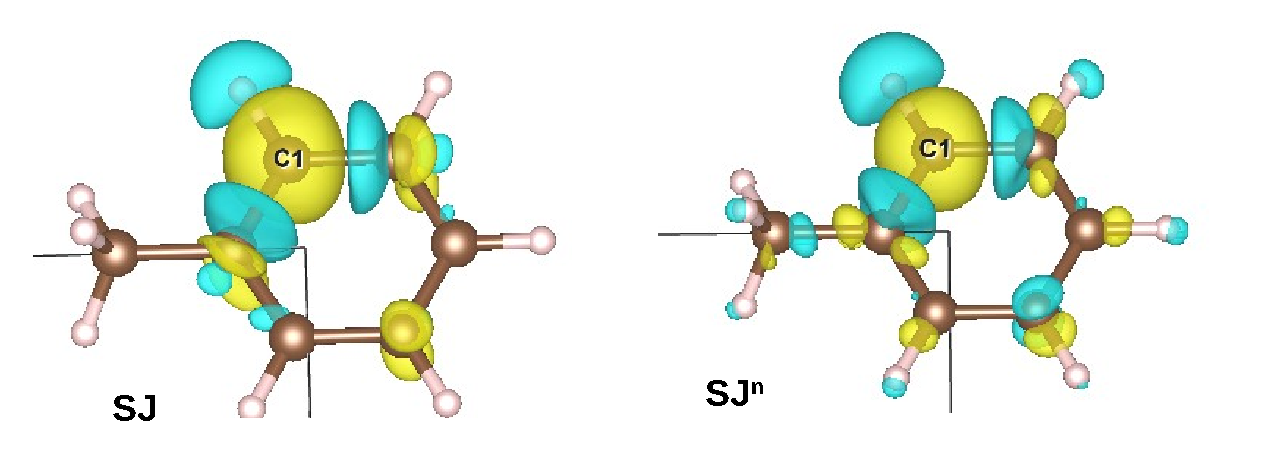
\includegraphics[width=\linewidth]{FigureS3}
\caption{Impact of the slab thickness (indicated as the number of layers, $N$) on the mean bulk (filled markers)  and surface (empty markers) \dbe{}, as computed with the SJ protocol and different references. The vertical lines indicates standard deviation.}
\label{fig:slabsthicknessSJ}
\end{figure}

\begin{figure}[!h]
\centering
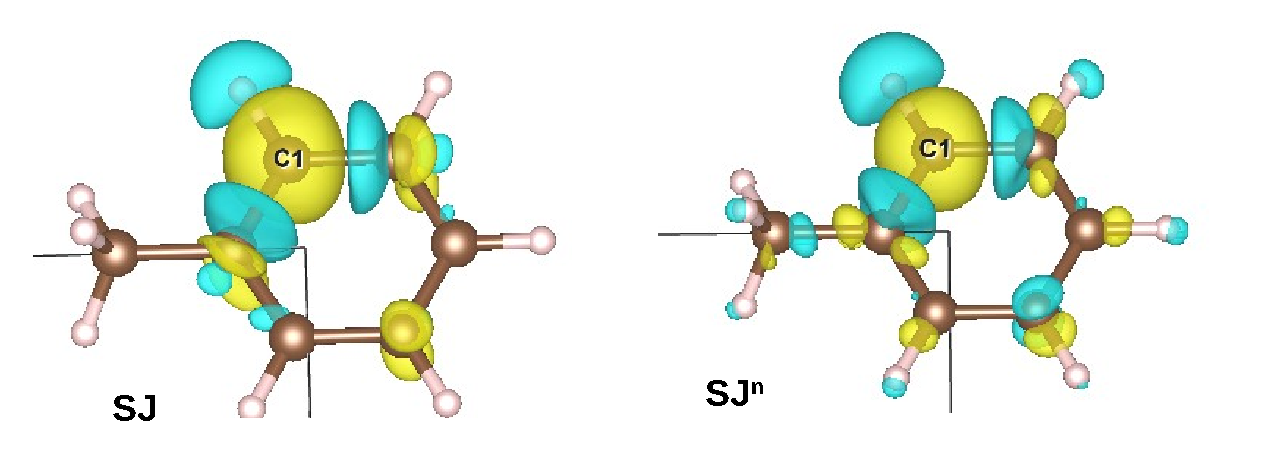
\includegraphics[width=\linewidth]{FigureS4}
\caption{Impact of the slab thickness (indicated as the number of layers) on the mean bulk (round markers)  and surface (square markers) \dbe{}, as computed with the SJ\textsuperscript{n} protocol and different references. The vertical lines indicates standard deviation.}
\label{fig:slabsthicknessSJn}
\end{figure}

\begin{table}
	\begin{tabular}{l cc c cc}
		\toprule
		& \multicolumn{2}{c}{Ca 2s} &&  \multicolumn{2}{c}{O 1s}\\
		\cline{2-3} \cline{5-6}
		& Bulk & Surface & & Bulk & Surface \\
		\midrule
		\multicolumn{6}{c}{$E_{ref}=0$}  \\
		\midrule
		Ca & 0.97 $\pm$ 0.04 & 1.44 $\pm$ 0.01 &  & --- & --- \\
		\ce{CaH2} & 1.00 $\pm$ 0.02 & 0.99 $\pm$ 0.00 &  & --- & --- \\
		CaO & -0.75 $\pm$ 0.02 & -0.13 $\pm$ 0.00 &  & -7.02 $\pm$ 0.02 & -7.54 $\pm$ 0.00 \\
		\ce{CaO.H2O} & -1.21 $\pm$ 0.06 & -0.68 $\pm$ 0.01 &  & -7.50 $\pm$ 0.06 & -5.83 $\pm$ 0.01 \\
		\midrule
		\multicolumn{6}{c}{$E_{ref}=E_F$} \\
		\midrule
	Ca & -0.09 $\pm$ 0.04 & 0.37 $\pm$ 0.01 &  & --- & --- \\
	\ce{CaH2} & 0.66 $\pm$ 0.02 & 0.50 $\pm$ 0.00 &  & --- & --- \\
	CaO & 0.31 $\pm$ 0.04 & 0.82 $\pm$ 0.00 &  & -2.99 $\pm$ 0.01 & -3.63 $\pm$ 0.00 \\
		\ce{CaO.H2O} & 0.30 $\pm$ 0.07 & 0.86 $\pm$ 0.01 &  & -2.97 $\pm$ 0.07 & -1.33 $\pm$ 0.01 \\
		\midrule
		\multicolumn{6}{c}{$E_{ref}=\varepsilon_{Ar,2s}$}  \\
		\midrule
		Ca & -0.07 $\pm$ 0.04 & 0.38 $\pm$ 0.00 &  & --- & --- \\
		\ce{CaH2} & -0.61 $\pm$ 0.02 & -0.62 $\pm$ 0.00 &  & --- & --- \\
		CaO & -0.88 $\pm$ 0.01 & -0.16 $\pm$ 0.00 &  & -3.55 $\pm$ 0.03 & -4.04 $\pm$ 0.00 \\
		\ce{CaO.H2O} & -0.97 $\pm$ 0.07 & -0.49 $\pm$ 0.07 &  & -3.83 $\pm$ 0.08 & -1.63 $\pm$ 0.72 \\
		\midrule
		\multicolumn{6}{c}{$E_{ref}=E_\infty$} \\
		\midrule
		Ca & -0.12 $\pm$ 0.04 & 0.37 $\pm$ 0.01 &  & --- & --- \\
		\ce{CaH2} & -0.63 $\pm$ 0.02 & -0.65 $\pm$ 0.00 &  & --- & --- \\
		CaO & -0.92 $\pm$ 0.00 & -0.20 $\pm$ 0.00 &  & -3.58 $\pm$ 0.03 & -4.05 $\pm$ 0.00 \\
		\ce{CaO.H2O} & -1.00 $\pm$ 0.06 & -0.47 $\pm$ 0.01 &  & -3.74 $\pm$ 0.06 & -2.04 $\pm$ 0.01 \\
		\midrule
		\multicolumn{6}{c}{$E_{ref}=\phi$}  \\
		\midrule
		Ca & 0.93 $\pm$ 0.04 & 1.44 $\pm$ 0.01 &  & --- & --- \\
		\ce{CaH2} & -0.28 $\pm$ 0.02 & -0.15 $\pm$ 0.00 &  & --- & --- \\
		CaO & -1.98 $\pm$ 0.03 & -1.16 $\pm$ 0.00 &  & -7.63 $\pm$ 0.05 & -7.95 $\pm$ 0.00 \\
		\ce{CaO.H2O} & -2.51 $\pm$ 0.05 & -2.01 $\pm$ 0.01 &  & -8.27 $\pm$ 0.06 & -6.54 $\pm$ 0.01 \\
		\bottomrule
		\end{tabular}
		    \caption{Mean (and standard deviation) bulk and surface \dbe{} values for 6-layer (Ca, CaO, and \ce{CaO.H2O}) and 12-layer (\ce{CaH2}) slabs, computed using the SJ protocol with various reference energies.}
\end{table}

\begin{table}
	\begin{tabular}{l cc c cc}
		\toprule
		& \multicolumn{2}{c}{Ca 2s} &&  \multicolumn{2}{c}{O 1s}\\
		\cline{2-3} \cline{5-6}
		& Bulk & Surface & & Bulk & Surface \\
		\midrule
		\multicolumn{6}{c}{$E_{ref}=0$}  \\
		\midrule
		Ca & 1.26 $\pm$ 0.04 & 1.73 $\pm$ 0.01 &  & --- & --- \\
		\ce{CaH2} & 1.75 $\pm$ 0.05 & 2.51 $\pm$ 0.00 &  & --- & --- \\
		CaO & 0.50 $\pm$ 0.05 & 1.22 $\pm$ 0.00 &  & -8.90 $\pm$ 0.06 & -9.03 $\pm$ 0.00 \\
		\ce{CaO.H2O} & 1.11 $\pm$ 0.07 & 2.32 $\pm$ 0.01 &  & -8.40 $\pm$ 0.05 & -6.38 $\pm$ 0.01 \\
		\midrule
		\multicolumn{6}{c}{$E_{ref}=E_F$}  \\
		\midrule
		Ca & -0.08 $\pm$ 0.03 & 0.38 $\pm$ 0.01 &  & --- & --- \\
		CaH2 & -0.33 $\pm$ 0.03 & 0.11 $\pm$ 0.00 &  & --- & --- \\
		CaO & -0.46 $\pm$ 0.05 & 0.39 $\pm$ 0.00 &  & -0.63 $\pm$ 0.14 & -0.79 $\pm$ 0.00 \\
		\ce{CaO.H2O} & -0.16 $\pm$ 0.18 & 1.02 $\pm$ 0.01 &  & -0.43 $\pm$ 0.15 & 1.67 $\pm$ 0.01 \\
		\midrule
		\multicolumn{6}{c}{$E_{ref}=\varepsilon_{Ar,2s}$}  \\
		\midrule
		Ca & 0.51 $\pm$ 0.04 & 0.99 $\pm$ 0.00 &  & --- & --- \\
		\ce{CaH2} & 0.01 $\pm$ 0.04 & 0.76 $\pm$ 0.01 &  & --- & --- \\
		CaO & 0.96 $\pm$ 0.09 & 1.51 $\pm$ 0.00 &  & -4.66 $\pm$ 0.01 & -5.00 $\pm$ 0.00 \\
		\ce{CaO.H2O} & 2.65 $\pm$ 0.05 & 3.50 $\pm$ 0.01 &  & -3.06 $\pm$ 0.11 & -1.42 $\pm$ 0.01 \\
		\midrule
		\multicolumn{6}{c}{$E_{ref}=E_F'$ }  \\
		\midrule
		Ca & 0.69 $\pm$ 0.04 & 1.15 $\pm$ 0.03 &  & --- & --- \\
		\ce{CaH2} & 1.41 $\pm$ 0.04 & 1.88 $\pm$ 0.00 &  & --- & --- \\
		CaO & -0.93 $\pm$ 0.10 & 0.09 $\pm$ 0.00 &  & -4.99 $\pm$ 0.19 & -4.93 $\pm$ 0.00 \\
		\ce{CaO.H2O} & -1.68 $\pm$ 0.28 & -0.16 $\pm$ 0.01 &  & -5.84 $\pm$ 0.23 & -3.40 $\pm$ 0.01 \\
		\bottomrule
	\end{tabular}
	\caption{Mean (and standard deviation) bulk and surface \dbe{} values for 6-layer (Ca, CaO, and \ce{CaO.H2O}) and 12-layer (\ce{CaH2}) slabs, computed using the SJ\textsuperscript{n} protocol with various reference energies.}
\end{table}

\newcommand{\XPSsa}[3]{
\begin{figure}[!h]
	\centering
	\includegraphics[width=.8\linewidth]{Figure#1a}
	\includegraphics[width=.8\linewidth]{Figure#1b}
	\caption{Difference (dotted line) between the XPS spectrum before (dashed line) and after (plain line) adsorption for compounds \textbf{#2} (top) and \textbf{#3} (bottom) on the different substrates. }
	\label{fig:spectraXPSads#2#3}
\end{figure}
}

\XPSsa{S5}{a}{b}
\XPSsa{S6}{c}{d}
\XPSsa{S7}{e}{f}
\XPSsa{S8}{g}{h}
\XPSsa{S9}{i}{j}

\begin{figure}[!h]
	\centering
	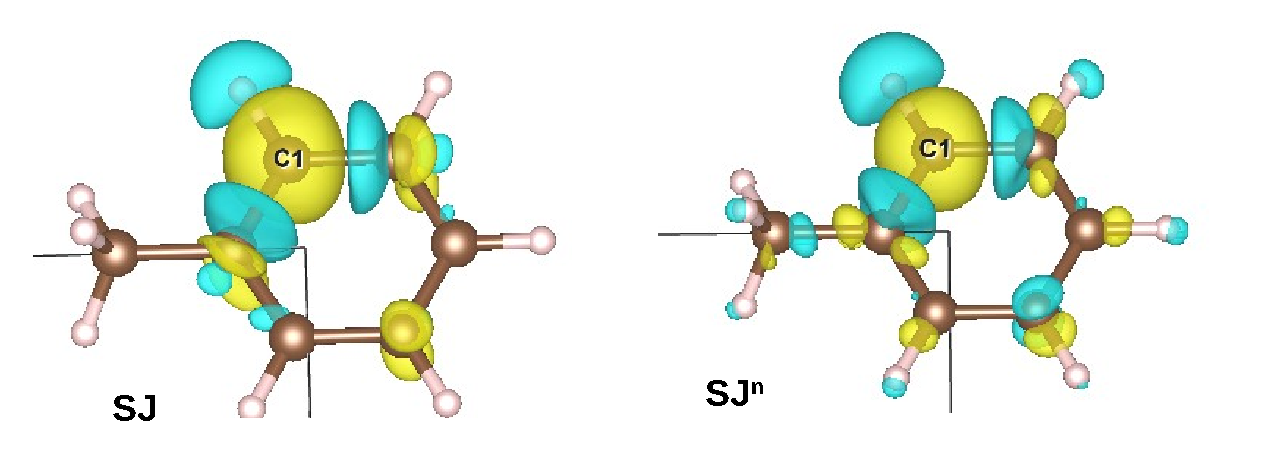
\includegraphics[width=.8\linewidth]{FigureS10}
	\caption{XPS spectra (as computed with the SJ\textsuperscript{n} protocol, using $\sigma=\SI{0.6}{\electronvolt}$) of the adsorbates \textbf{h} and \textbf{j} on Ca, CaO and \ce{CaO.H2O}.}
	\label{fig:possSJn}
\end{figure}

\clearpage
\bibliography{biblio}
	
\end{document}